\section{Analysis and Design}

In this chapter, the aims are to:

\begin{itemize}
    \item Provide a high-level overview of the design of the system to estimate blood pressure values from PPG signals
    \item Describe the specifications of each stage of the system based on the findings of the literature review in Chapter 2
    \item Discuss any changes or justifications for design choices made for the system blocks where appropriate
\end{itemize}

\subsection{High Level overview of proposed design}
Figure \ref{blockdiag} illustrates the high-level design specification for the 
cuffless estimation of blood pressure from PPG signals. The diagram describes 
each discrete stage that is required. 

\begin{figure}[H]
    \centering
    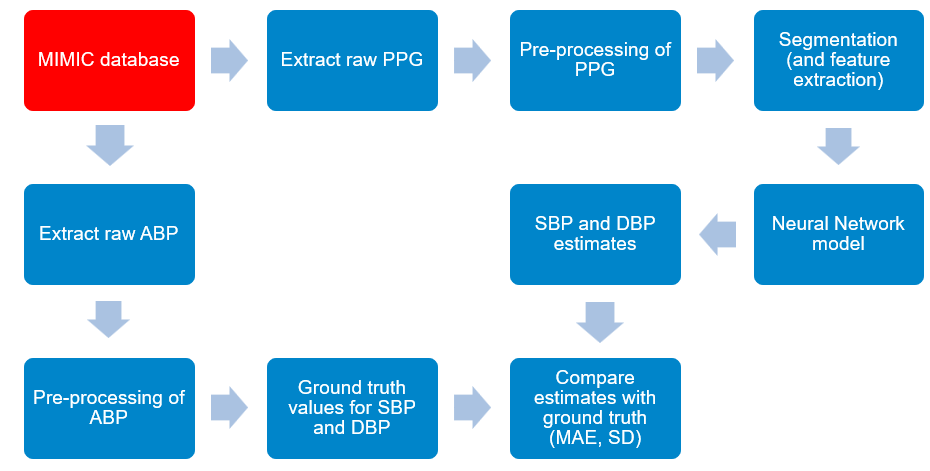
\includegraphics[width=15cm,height=15cm,keepaspectratio]{AnalysisDesign/blockDiag.png}
    \caption{High-level block diagram of blood pressure cuffless estimation from PPG}
    \label{blockdiag}
\end{figure}\noindent The following subchapters will explain each stage in more detail.

\subsection{Choice of database}
As previously discussed in the literature review in Chapter 2, the 
MIMIC (Multi-parameter Intelligent Monitoring for Intensive Care) database has been chosen 
for the implementation. The data has been recorded from patient monitors in the medical, 
surgical, and cardiac intensive care units of Boston's Beth Israel Hospital. The MIMIC Database 
has records for 72 ICU patients. Referring back to the motivation for this FYP, the early detection and prevention of hypertension and other Cardiovascular diseases (CVDs) is 
crucial. Therefore, testing was only performed on patients with CVDs or heart-related issues, which was a data subset of 12 patients. The age range of the patients 
is 52 to 85 years. In addition, the data is from 8 males and 4 females. The data obtained from the bedside monitors are divided into files 
each containing 10 minutes of recorded signals, which can then be assembled without 
gaps to form a continuous recording \cite{Moody1996}. Both the PPG and ABP signals in the MIMIC database 
are sampled at a frequency of $125$ Hz. Each patient record contains a minimum of 73 and a maximum of 412 individual files.
 The patients contain one of the following heart-related diseases:
\begin{itemize}
    \item \textbf{Congestive Heart Failure} (CHF). This refers to patients who suffer a chronic progressive condition that affects the pumping power of your heart muscle
    \item \textbf{Postoperative Coronary Artery Bypass Graft} (CABG). This refers to patients recovering from a surgical procedure to restore normal blood flow to an obstructed coronary artery
    \item \textbf{Myocardial Infarction} (MI) / \textbf{Cardiogenic shock}. This refers to patients who have suffered heart attacks or cardiac shock
\end{itemize}NEED REFERENCES HERE!


\subsection{Choice of programming language}
Python is used as the sole programming language for this project. Python has a wide 
variety of easy to use and powerful libraries \cite{Python}. The scientific libraries from Python 
that are used for this project are \texttt{numpy} \cite{numpy} and \texttt{pandas} \cite{pandas}. In addition, the 
machine learning libraries used are \texttt{tensorflow} \cite{tensorflow}, \texttt{keras} \cite{keras} and \texttt{scikit-learn} \cite{scikit}. 
In addition the \texttt{heartpy} \cite{heartpy} and \texttt{wfdb-python} \cite{wfdb} packages were installed, which are libraries of 
tools for reading, writing, and processing Waveform-Database (WFDB) signals and annotations. \\ \newline \noindent MATLAB was also 
considered as a potential programming language to use, due to it having a wide range of 
signal processing and machine learning add-on toolboxes. However Python has been shown 
to offer a wider set of choices in graphics packages and toolsets, such as 
through \texttt{matplotlib} \cite{matplotlib}, and it also produces more compact and readable 
code. For this FYP, Python will be used in the Google Colaboratory environment in the form of a Jupyter notebook, as there is access to 
to high-performance Graphics Processing Units (GPUs) on Google Cloud for training using machine learning. 


\subsection{Extraction of raw signal data}
For this implementation, it is necessary to extract the raw signal data 
for two signals, the ABP and PPG. Both signals are first extracted from 
the Physionet website using the \texttt{wfdb} package.
\begin{itemize}
    \item Use heartpy library (hp.process)
    \item Despite being measured using gold-standard invasive, still needs preprocessing. TALK ABOUT ALL STEPS!
\end{itemize}


\subsection{Pre-processing of PPG}
\begin{itemize}
    \item hp.process
    \item Butterworth filter
    \item Z-normalisation
    \item Additional sanity checks using custom SBP and DBP min and max values
\end{itemize}

The $Z$-score normalisation equation is applied to the PPG signal, 
\begin{equation}
    Z_{i} = \frac{(PPG_{i} - \mu_{PPG_i}) }{\sigma_{PPG_i}}
\end{equation} \noindent where $Z_{i}$ is the $Z$-score normalised PPG signal for a particular window $i$, 
$PPG_{i}$ is the raw PPG signal, $\mu$ is the mean of the PPG signal and $\sigma$ is the standard deviation.


\subsection{Feature extraction}
\begin{itemize}
    \item Based on Literature review, machine learning methods are favouring automated feature extraction
    \item Hence, this method will segment the PPG signal into discrete windows and feed this into the network
    \item However, there is still prominence among the handcrafted feature methods
    \item Provide an additional exploration to add the first and second derivatives of the PPG to see if this affects the accuracy for any model
\end{itemize}

\subsection{Machine Learning models}
\begin{itemize}
    \item Function based for each ML model
    \item Using tensorflow and keras
\end{itemize}


\subsection{Error metrics}
The two considered error calculations used in this experimentation are the Mean Absolute Error 
(MAE) and Root Mean Square Error (RMSE). They are defined by the following equations, 
\begin{align}
    MAE &= \frac{1}{N} \sum_{i=1}^N \lvert a_{i_{M}} - b_{i_{M}} \rvert \\
    RMSE &= \frac{1}{N} \sqrt{\sum_{i=1}^N \lvert a_{i_{M}} - b_{i_{M}} \rvert^2}
\end{align}\noindent In the context of BP estimation, $b_{i_{M}}$ and $a_{i_{M}}$ represent the true 
value and BP estimate respectively for the $M$th element of the time sequence.
